\chapter{第一部分}
\section{问题概述}
%
%%对问题的直观描述
%
该部分包含第1,2小题,要求完成以下任务:
\begin{enumerate}
    \item 利用Expr类表示由以下语句形成的合取式
    \begin{enumerate}
        \item \begin{itemize}
            \item $A\lor B$
            \item $\lnot A\leftrightarrow (\lnot B\lor C)$
            \item $\lnot A\lor \lnot B\lor C$
        \end{itemize}
        \item \begin{itemize}
            \item $C\leftrightarrow (B\lor D)$
            \item $A\rightarrow (\lnot B\land \lnot D)$
            \item $\lnot(B\land\lnot C)\rightarrow A$
            \item $\lnot D\rightarrow C$
        \end{itemize}
    \end{enumerate}
    \item 用PropSymbolExpr类构造符号,并形成含有以下语义的逻辑语句,最终连接形成合取式
    \begin{enumerate}
        \item Pacman is alive at time 1 if and only if he was alive at time 0 and he was not killed at time 0 or he was not alive at time 0 and he was born at time 0.
        \item At time 0, Pacman cannot both be alive and be born.
        \item Pacman is born at time 0.
    \end{enumerate}
    \item 补全findModelCheck函数,使得它的返回值和findeModel(Expr('a'))一致。该问题考察的是对于findModel函数功能的理解
    \item 补全entails函数,其功能是判断给定前提是否蕴含指定结论
    \item 补全plTrueInverse函数,其功能是判断给定赋值是否满足所给语句的否定。
    \item 补全atLeastOne函数,其功能是接受一列文字,返回一个合取式,该合取式为真当且仅当给定文字中至少有一个文字为真
    \item 补全atMostOne函数,其功能是接受一列文字,返回一个合取式,该合取式为真当且仅当给定文字中至多有一个文字为真
    \item 补全exactlyOne函数,其功能是接受一列文字,返回一个合取式,该合取式为真当且仅当给定文字中恰好有一个文字为真
\end{enumerate}
在补全atLeastOne,atMostOne,exactlyOne函数中,不允许调用to\_cnf及其相关函数。
%
%对项目已有代码的阅读和理解
%

%
%解决问题的思路和想法
%

\section{算法设计}
%
%用自己的语言描述解决问题所使用的算法的原理及功能,设计思路和算法流程图
%
满足由单一文字构成的表达式的模型仅由一个True组成。

判断蕴含关系可以使用反证法,即只需要判断所给前提和所给结论的否定所形成的合取式是否为可满足式即可。如果时,则说明蕴含关系不成立,否则成立。

给定一列文字,其中至少有一个为真当且仅当他们的析取式为真,而由于文字之间的析取式作为整体时可以视为合取式,所以atLeastOne函数只需要返回给定文字的合取式即可。

给定一列文字,其中至多有一个为真当且仅当任意两个文字之间的合取式不为真,为了转换为合取式,需要利用德摩根律,转化为任意两个文字的否定之间的析取式为真。

给定一列文字,其中恰好有一个为真当且仅当其中至少有一个为真且其中至多有一个为真。
\section{算法实现}
在完成该项目的全部过程中,为了便于调试并且与autograder的答案匹配,均调用conjoin和disjoin函数来分别构造合取式和析取式,而不是使用\&和|运算符。

在完成任务1时,我从logic.py中引入了SpecialExpr类,来表示简化代码。

由于findModel以\{符号:赋值\}的形式返回满足给定合取式的模型,所以,首先要构造'a'对应的符号,而这可以用提供的dummyClass实现,然后将其对应的值设为True即可。

实现plTrueInverse时,只需调用提供的plTrue函数,将参数inverse\_statement的否定作为参数输入即可。

在实现atMostOne时,借助combinations生成器来遍历给定文字的所有二组合。
%
%在算法原理的基础上,结合代码,讲述算法的实现细节、核心函数、模块输入输出,数据结构定义等内容
%
\begin{lstlisting}[emph={[3]sentence,premise,conclusion,assignments,inverse,statement,literals},emphstyle={[3]\color{vscode_parametercolor}},emph={[4]dummyClass,Expr,Dict,List},emphstyle={[4]\color{vscode_classcolor}}]
from logic import SpecialExpr

TRUE, FALSE = tuple(map(SpecialExpr, ['TRUE', 'FALSE']))
ZERO, ONE, TWO = tuple(map(SpecialExpr, [0, 1, 2]))
A, B, C, D, E, F, G, P, Q = tuple(map(Expr, 'ABCDEFGPQ'))
    
def sentence1() -> Expr:
    return conjoin([
        disjoin([A, B]),
        (~ A % disjoin([~ B, C])),
        disjoin(~ A, ~B, C)
    ])

def sentence2() -> Expr:
    return conjoin([
        C % disjoin([B, D]),
        A >> (conjoin([~B, ~D])),
        ~conjoin([B, ~C]) >> A,
        ~D >> C
    ])

def sentence3() -> Expr:
    PacmanAlive_0 = PropSymbolExpr('PacmanAlive', time=0)
    PacmanAlive_1 = PropSymbolExpr('PacmanAlive', time=1)
    PacmanBorn_0 = PropSymbolExpr('PacmanBorn', time=0)
    PacmanKilled_0 = PropSymbolExpr('PacmanKilled', time=0)
    return conjoin([
        PacmanAlive_1 % disjoin([conjoin([PacmanAlive_0, ~PacmanKilled_0]), conjoin(~PacmanAlive_0, PacmanBorn_0)]),
        ~conjoin([PacmanAlive_0, PacmanBorn_0]),
        PacmanBorn_0
    ])

def findModelCheck() -> Dict[Any, bool]:
    class dummyClass:
        def __init__(self, variable_name: str = 'A'):
            self.variable_name = variable_name

        def __repr__(self):
            return self.variable_name
    return {dummyClass('a'): True}

def entails(premise: Expr, conclusion: Expr) -> bool:
    return findModel(conjoin([premise, ~conclusion])) == False

def plTrueInverse(assignments: Dict[Expr, bool], inverse_statement: Expr) -> bool:
    return pl_true(~inverse_statement, assignments)

def atLeastOne(literals: List[Expr]) -> Expr:
    return disjoin(literals)  # 已经能够保证是合取式

from itertools import *

def atMostOne(literals: List[Expr]) -> Expr:
    return conjoin([disjoin([~atom1,~atom2]) for atom1,atom2 in combinations(literals, 2)])

def exactlyOne(literals: List[Expr]) -> Expr:
    return conjoin( [atLeastOne(literals) ,atMostOne(literals)])
\end{lstlisting}
\section{实验结果}
%
%对试验结果进行详细展示,对每个问题展示测试截图,对于测试用例进行描述说明,对于为通过测试的用例结合自己的算法进行分析,可以结合调试过程进行分析
%
成功通过Question1和Question2的全部测试,实验结果截图见图\ref{q12}。
\begin{figure}[!htbp]
    \centering
    \begin{minipage}[t]{0.4\textwidth}
    \centering
    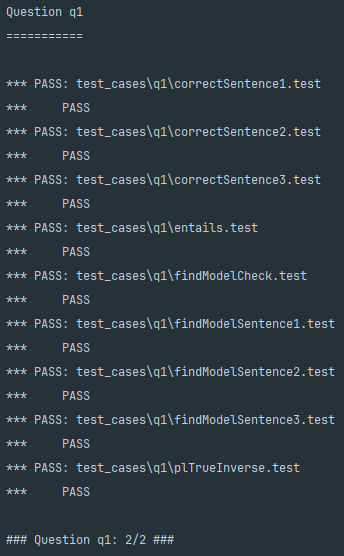
\includegraphics[width=\textwidth]{pic/q1.png}
    \end{minipage}
    \begin{minipage}[t]{0.4\textwidth}
    \centering
    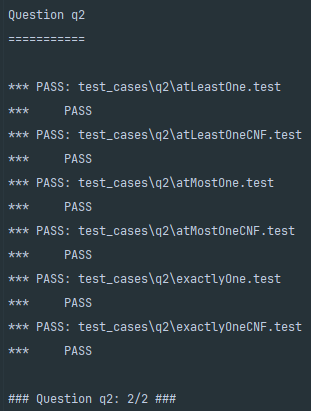
\includegraphics[width=\textwidth]{pic/q2.png}
    \end{minipage}
    \caption{Question1\&2实验结果}\label{q12}
\end{figure}
这里所使用的到的测试用例较为基础,检查了上述函数是否能够返回正确的结果。
其中,对于atLeastOne,atMostOne和exactlyOne这三个函数的检测方式是检验包含不同数量的True的模型是否满足由函数返回的表达式。
%
%实验中遇到的问题及解决方案,收获和思考:对算法的理解、优缺点的评价、算法的适用场景
%
